%%
%% This is file `sample-sigconf.tex',
%% generated with the docstrip utility.
%%
%% The original source files were:
%%
%% samples.dtx  (with options: `sigconf')
%% 
%% IMPORTANT NOTICE:
%% 
%% For the copyright see the source file.
%% 
%% Any modified versions of this file must be renamed
%% with new filenames distinct from sample-sigconf.tex.
%% 
%% For distribution of the original source see the terms
%% for copying and modification in the file samples.dtx.
%% 
%% This generated file may be distributed as long as the
%% original source files, as listed above, are part of the
%% same distribution. (The sources need not necessarily be
%% in the same archive or directory.)
%%
%% Commands for TeXCount
%TC:macro \cite [option:text,text]
%TC:macro \citep [option:text,text]
%TC:macro \citet [option:text,text]
%TC:envir table 0 1
%TC:envir table* 0 1
%TC:envir tabular [ignore] word
%TC:envir displaymath 0 word
%TC:envir math 0 word
%TC:envir comment 0 0
%%
%%
%% The first command in your LaTeX source must be the \documentclass command.
\documentclass[sigconf, anonymous=true]{acmart}

\usepackage{tabularray}
\UseTblrLibrary{booktabs}
%% NOTE that a single column version is required for 
%% submission and peer review. This can be done by changing
%% the \doucmentclass[...]{acmart} in this template to 
%% \documentclass[manuscript,screen]{acmart}
%% 
%% To ensure 100% compatibility, please check the white list of
%% approved LaTeX packages to be used with the Master Article Template at
%% https://www.acm.org/publications/taps/whitelist-of-latex-packages 
%% before creating your document. The white list page provides 
%% information on how to submit additional LaTeX packages for 
%% review and adoption.
%% Fonts used in the template cannot be substituted; margin 
%% adjustments are not allowed.

%%
%% \BibTeX command to typeset BibTeX logo in the docs
\AtBeginDocument{%
  \providecommand\BibTeX{{%
    \normalfont B\kern-0.5em{\scshape i\kern-0.25em b}\kern-0.8em\TeX}}}

%% Rights management information.  This information is sent to you
%% when you complete the rights form.  These commands have SAMPLE
%% values in them; it is your responsibility as an author to replace
%% the commands and values with those provided to you when you
%% complete the rights form.
\setcopyright{acmcopyright}
\copyrightyear{2018}
\acmYear{2018}
\acmDOI{XXXXXXX.XXXXXXX}

%% These commands are for a PROCEEDINGS abstract or paper.
\acmConference[Conference acronym 'XX]{Make sure to enter the correct
  conference title from your rights confirmation emai}{June 03--05,
  2018}{Woodstock, NY}
%
%  Uncomment \acmBooktitle if th title of the proceedings is different
%  from ``Proceedings of ...''!
%
%\acmBooktitle{Woodstock '18: ACM Symposium on Neural Gaze Detection,
%  June 03--05, 2018, Woodstock, NY} 
\acmPrice{15.00}
\acmISBN{978-1-4503-XXXX-X/18/06}


%%
%% Submission ID.
%% Use this when submitting an article to a sponsored event. You'll
%% receive a unique submission ID from the organizers
%% of the event, and this ID should be used as the parameter to this command.
%%\acmSubmissionID{123-A56-BU3}

%%
%% For managing citations, it is recommended to use bibliography
%% files in BibTeX format.
%%
%% You can then either use BibTeX with the ACM-Reference-Format style,
%% or BibLaTeX with the acmnumeric or acmauthoryear sytles, that include
%% support for advanced citation of software artefact from the
%% biblatex-software package, also separately available on CTAN.
%%
%% Look at the sample-*-biblatex.tex files for templates showcasing
%% the biblatex styles.
%%

%%
%% The majority of ACM publications use numbered citations and
%% references.  The command \citestyle{authoryear} switches to the
%% "author year" style.
%%
%% If you are preparing content for an event
%% sponsored by ACM SIGGRAPH, you must use the "author year" style of
%% citations and references.
%% Uncommenting
%% the next command will enable that style.
%%\citestyle{acmauthoryear}

%%
%% end of the preamble, start of the body of the document source.
\begin{document}

%%
%% The "title" command has an optional parameter,
%% allowing the author to define a "short title" to be used in page headers.
\title{Few-Shot Learning of Intents Without Training Classifiers}

%%
%% The "author" command and its associated commands are used to define
%% the authors and their affiliations.
%% Of note is the shared affiliation of the first two authors, and the
%% "authornote" and "authornotemark" commands
%% used to denote shared contribution to the research.
\author{Martin Dimkovski}
\authornote{Both authors contributed equally to this research.}
\affiliation{%
  \institution{Intact Financial Corp.}
%   \streetaddress{P.O. Box 1212}
  \city{Toronto}
  \state{ON}
  \country{Canada}
%   \postcode{43017-6221}
}
\email{martin.dimkovski@intact.net}

\author{Wei Yuan}
\authornotemark[1]
\affiliation{
  \institution{York University}
%   \streetaddress{1 Th{\o}rv{\"a}ld Circle}
  \city{Toronto}
  \state{ON}
  \country{Canada}
  }
\email{wyuancs@yorku.ca
}
\author{Aijun An}
\affiliation{%
  \institution{York University}
  \city{Toronto}
  \state{ON}
  \country{Canada}
}
\email{aan@eecs.yorku.ca}

%%
%% By default, the full list of authors will be used in the page
%% headers. Often, this list is too long, and will overlap
%% other information printed in the page headers. This command allows
%% the author to define a more concise list
%% of authors' names for this purpose.
% \renewcommand{\shortauthors}{Trovato and Tobin, et al.}

%%
%% The abstract is a short summary of the work to be presented in the
%% article.
\begin{abstract}
We present an application of language-embedding models to intent detection for an enterprise dialogue system. We show that it is possible to meet and exceed state-of-the-art results in resolving conversation intents without training classifiers, in particular when there is only a few examples per intent or as little as one. By manipulating text embedding spaces, intents are resolved through semantic similarities between the user utterance and intent examples or intent superset descriptions. Our results show that off-the-shelf embedding models can work reasonably well in production without fine-tuning, and that they are relatively easy to fine-tune as data becomes available. 
\end{abstract}

%%
%% The code below is generated by the tool at http://dl.acm.org/ccs.cfm.
%% Please copy and paste the code instead of the example below.
%%
\begin{CCSXML}
<ccs2012>
 <concept>
  <concept_id>10010520.10010553.10010562</concept_id>
  <concept_desc>Computer systems organization~Embedded systems</concept_desc>
  <concept_significance>500</concept_significance>
 </concept>
 <concept>
  <concept_id>10010520.10010575.10010755</concept_id>
  <concept_desc>Computer systems organization~Redundancy</concept_desc>
  <concept_significance>300</concept_significance>
 </concept>
 <concept>
  <concept_id>10010520.10010553.10010554</concept_id>
  <concept_desc>Computer systems organization~Robotics</concept_desc>
  <concept_significance>100</concept_significance>
 </concept>
 <concept>
  <concept_id>10003033.10003083.10003095</concept_id>
  <concept_desc>Networks~Network reliability</concept_desc>
  <concept_significance>100</concept_significance>
 </concept>
</ccs2012>
\end{CCSXML}

\ccsdesc[500]{Computer systems organization~Embedded systems}
\ccsdesc[300]{Computer systems organization~Redundancy}
\ccsdesc{Computer systems organization~Robotics}
\ccsdesc[100]{Networks~Network reliability}

%%
%% Keywords. The author(s) should pick words that accurately describe
%% the work being presented. Separate the keywords with commas.
\keywords{datasets, neural networks, gaze detection, text tagging}

%% A "teaser" image appears between the author and affiliation
%% information and the body of the document, and typically spans the
%% page.

%%
%% This command processes the author and affiliation and title
%% information and builds the first part of the formatted document.
\maketitle

\section{Introduction}
Task-oriented dialogue systems \cite{zhang2020recent}, such as chatbot and question-answering systems, allow users to interact with systems using natural language to solve particular tasks or get information. The goal of the system is to map user inputs into correct \textit{intents} which then trigger predefined actions. 

The dominant method for predicting the intent in dialogue systems is to use text classifiers $\math{f(u)}$ which map the user input $\math{u}$ into a closed set of $\math{K}$ intents $\math{\{I_1, I_2,...I_K\}}$ \cite{intent_classification_for_dialogue_uterances}. Each classifier needs to be trained before the system can be used. This requires collecting enough labeled training data from subject matter experts or real user examples in the form of $\math{(u, I)}$ pairs of user inputs and intents. To make changes after training, such as adding or deleting an intent, the classifiers need to be retrained. 

The constraints with the dominant method can be illustrated by imagining a new deployment where the intents $\math{\{I_1, I_2,...I_K\}}$ are known with minimal initial information such as a single example per intent or a short description. This would be sufficient for a human to start matching new user inputs to the intents. However, a classifier of the form $\math{f(u)=>\{I_1, I_2,...I_K\}}$ would typically need more data before it can be trained. Further, if a new intent $\math{I_{K+1}}$ needs to be added, the system needs to be stopped and $\math{f(u)}$ retrained to map into $\math{\{I_1, I_2,...I_K, I_{K+1}\}}$.

An obvious alternative would be to use a semantic similarity function $\math{sim(u, I)}$ which can score the similarity between the user input $\math{u}$ and each intent, after which the most similar intent can be chosen. Such a function could be pre-trained on the language as a whole or text collections from narrower problem domains, and be usable even without requiring application-specific training data, unlike classifiers. As training data becomes available, the similarity function can be further optimized. Changing or adding intents can be done online, without disrupting the system. 

Until recently, using similarity functions as above has been impractical. If the language model is called every time the $\math{sim(u, I)}$ function runs, the inference time would scale proportional to the total number of intent examples. In realistic dialogue systems, this would make the inference time hundreds or thousands of times longer than using a $\math{f(u)}$ classifier. A known alternative, instead of training language models to output similarity scores, is to train them to embed text into vector spaces where semantic similarity translates into geometric proximity. We will refer to these as embedding-optimized language models (ELMs). Using ELMs, the language model has to run only once to get the embedding of the user input $\math{u}$, after which the similarity function is a matrix operation with pre-computed intent embeddings. This results in inference time comparable to using classifiers. Nevertheless, previous ELM methods have not been shown to match the performance and scalability of classifiers as methods for intent resolution. 

The last few years have seen innovations ELMS based on Transformer-based architectures specialized to produce effective text embeddings as their final output \citep{cer2018universal, reimers-2019-sentence-bert, gao2021simcse}. Our key research question is whether the latest ELMs can match classifiers as methods for intent resolution, thereby removing the classifier constraints described above. In other words, whether dialogue systems can gain the benefits of needing considerably less training data, especially for initial launches, and being able to change or add intents online without retraining interruptions, all of this without losing on performance and scalability. 

In this paper, we provide evidence suggesting that the latest ELMs can outperform classifiers in few-shot learning scenarios where the number of examples per intent is 10 or less. Our results top the scores across leading benchmark datasets for few-shot learning. We also present a ELM-based production system in a large enterprise setting which operates with as little as one example per intent. We shows that even without any fine-tuning on training data, some off-the-shelf ELMs can work reasonably well for immediate use. We also present some interpretability and malleability benefits from using an optional intent tree structure which is particularly enabled by an ELM approach. 


\begin{figure}[ht]
  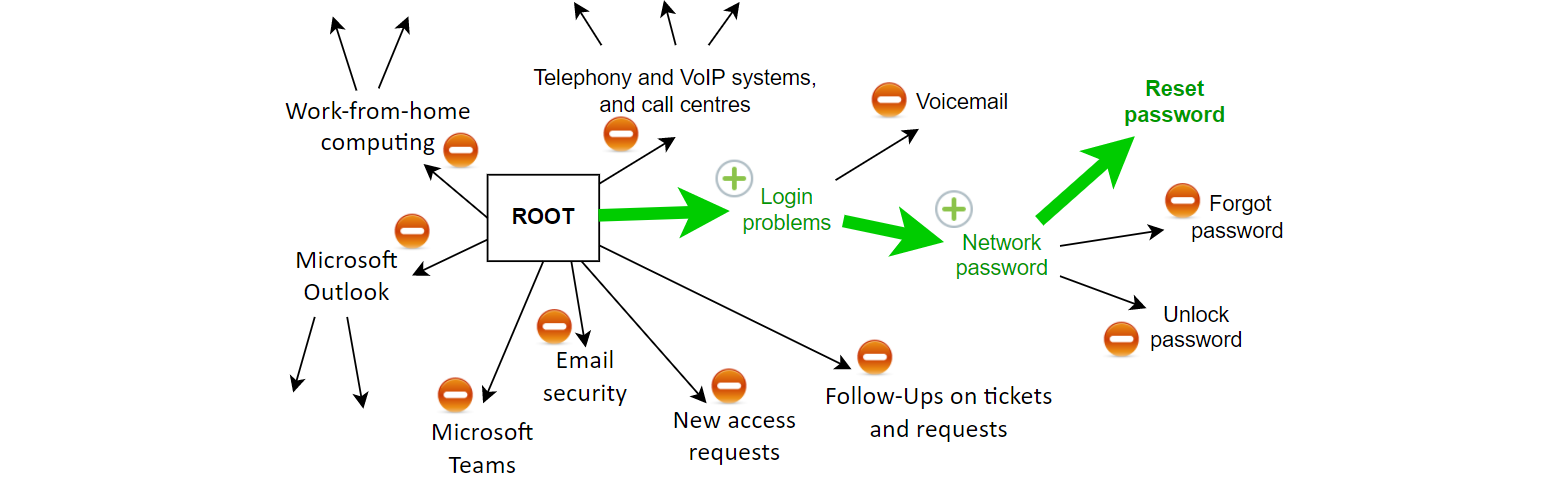
\includegraphics[width=\columnwidth]{pic/figure1.PNG}
  \caption{Part of the intent tree related to the "reset password"}
\end{figure}


\section{Deployed ELM-based Approach}
We developed and deployed an ELM-based dialogue system for the helpdesk operations at Intact Financial Corp., the largest provider of property and casualty insurance in Canada and a leading provider of global specialty insurance. While Intact also uses classifier-based dialogue systems, this ELM-based approach was motivated by the desire to train a single domain-specific language model for embeddings so they can be used not only for resolving intents, but also for topic detection, clustering, and other NLP tasks. Another motivation was to get started with as little as a single or a few examples per intent. The ELM-based intent resolver powers a chatbot that has served over 53K conversations since its deployment a year ago.

\subsection{Overview of the Dialogue System}
\label{chabotOverview}
The chatbot uses a custom dialogue state machine which can prompt the user for clarification if required information is missing. The state machine is multi-turn and guides the dialogue along possible paths in an intent tree structure, where each leaf node is a final or most specific intent, while each non-leaf node represents a superset of all final intents beneath it. Figure 1 shows an extract from an intent tree. The text content of leaf nodes is a set of all examples associated with that final intent in the dataset. The text content of a non-leaf node is additional information describing that superset and is created by knowledge base administrators. It is a summary of what all its descendant final intents are generally about. It might or might not contain any of the language used in the final intents examples.  

The user is not necessarily aware of all the branching events, i.e. dialogue turns. If the user input contains enough information for a confident decision at every superset node along a path to a leaf node, the dialogue engine ends up returning the final action or final answer in one turn. If the engine is not confident at any superset node, it queries the user for additional information before retrying to find path to a leaf node. 

Our design uses the intent tree for interpretability. It allows domain experts to organize knowledge by organizing answers under any hierarchy that is visually meaningful to them, while the training pairs are created automatically from the hierarchy as described below. The tree also offers interpretability to end users. If the dialogue engine fails in a final answer, the user can be shown what are the assumptions made by the chatbot, i.e. the branching decisions along the tree path. The engine allows the user to backtrack and instruct the bot in correcting any of the assumptions before retrying. Figure 2 shows a view of the user interface, after the user instructed the dialogue engine that the offered answer was not good. The engine retries and asks the user to clarify the branching choice at a node where the engine has low confidence. The choices we see in the option bubbles are the possible branches at that node. 

Under a conventional approach with intent classifiers, the system would either need a large classifier that can model all the final intents, or sets of intents would be organized somehow (e.g. in a tree) and each set would need its own classifier. Using ELMs, we use the same model at every turn, i.e. branching point in the intent tree. And because all text embeddings for a dataset can be pre-computed, only the user input has be processed through a deep network at inference, compared to the slower processing of multiple deep networks if the system were to use multiple classifier models. 

Our system allows for any number of examples to be linked to a final intent, and for multiple descriptions to be linked to a superset. In such cases, the example or description with the best similarity score to the user input will represent the leaf or non-leaf node. All nodes in production have less than 8 examples, with the average being 2.6, i.e. the system is few-shot at most and often only one-shot. 

\subsection{Branching Decision Making}

Given an ELM with an embedding dimensionality $\math{d}$, a user input $\math{u}$, and $\math{M}$ options represented by the text strings $\math{b_1, b_2, ... b_M}$ at a particular branching point on a path along the intent tree, the dialogue engine does the following: (i) calls the ELM to embed the text $\math{u}$ into an $\math{ELM(u)} \in \mathbb{R}^{d}$ vector if this is the first time it sees $\math{u}$ or if $\math{u}$ has changed; (ii) it then retrieves the $\math{ELM(b_1), ELM(b_2), ... ELM(b_M)}$ $\mathbb{R}^{d}$ vectors that are pre-computed and change only when the knowledge base is edited; (iii) makes a branching choice as 
\begin{equation*}
\arg\max_{b_x} Sim(\math{ELM(u)},\math{ELM(b_x)})
\end{equation*}
\noindent where the $\math{Sim}$ is a similarity function. In summary, each branching decision is a nearest-neighbour calculation over the embedded vectors. By repeating this process at each successive branching point, a path is found in the intent tree ending with a leaf node. 

This system uses SBERT\footnote{\url{https://github.com/UKPLab/sentence-transformers}} \citep{reimers-2019-sentence-bert} as the framework and library for ELMs. The first chatbot version was deployed in production without any fine-tuning, because the publicly available general purpose ELMs worked well enough for the first set of intents. We were also able to keep adding new intents without having to do anything for the ELM. As training data became available, the ELM began to be fine-tuned for increasingly better performance. 

\subsection{ELM Fine-tuning}
\label{ELMFineTuning}
The intent tree is used to automatically generate the fine-tuning pairs. Starting from a leaf node, i.e. a final intent, positive similarity pairs are created by pairing its examples with the superset description of its parent, then with its grandparent, and so on up until the root. An example for positive pairs for "reset password" is shown visually in Figure 1 and the exact pairs are listed in Appendix \ref{sec:posNegPairsExamples}. In summary, this creates positive associations from the root towards the leaf node. Negative similarity pairs are created by pairing the examples of a final intent leaf node with the superset descriptions of the siblings of its parent, then with the siblings of its grandparent, and so on as Figure 1 and Appendix \ref{sec:posNegPairsExamples} show in more details. These negative associations try to keep the intent inference along the correct ancestry path.

Using the above approach, we have found that fine-tuning is a straightforward process, without much sensitivity to learning rates, batch sizes, or number of epochs, as shown further below. Generally, the fine-tuning converges within a few epochs. 

\subsection{New Intents and Out-of-scope Function}
The automated nature of this fine-tuning pairs creation lets domain admins add new intents simply by visually creating a new leaf node, or visually changing the tree structure on the fly.  

Taking advantage of the flexibility of the ELM approach, we also developed a custom out-of-scope function. It measures the distance of a user input to cluster centroids of intent supersets and then compares these distances to the average inter-superset distance. In other words, it tries to estimate if the input is outside the manifold of the domain. If an input is much further compared to the inter-density, it is considered as an out-of-scope request. We have also found that a simpler out-of-scope function can be made just by creating an intent whose examples are picked solely on the quality of being far outside the domain. Multiple out-of-scope functions can be used across different branches of the intent tree. 


\section{Evaluation}
We evaluate first with public ELMs, which are already pre-trained for general use and can be used without any fine-tuning. Then we experiment with how much fine-tuning is need to approach state-of-the-art performance. The code for this paper is made publicly available. 

All the variations of our approach use the general form of an ELM combined with some similarity function over the embedding vectors. We will refer to this as the ELM+Sim approach. We vary some design choices in terms of the ELM and the similarity function. In one variation we calculate similarity between the user input and each example of a final intent, and then use nearest-neighbour as a representative measure for that intent. When the ELM is based on SBERT for example, we will label this variation as SBERT+NN. Another variation calculates the average of all the embeddings under an intent to get a single-vector representation. Then we can compare a user input to this average instead of the multiple calculation required with nearest-neighbour. We will refer to this as SBERT+AveSE. The latter variation makes the inference time proportional to number of intents instead of proportional to the total number of examples.  

We also replace SBERT as an ELM framework with SimCSE\footnote{\url{https://github.com/princeton-nlp/SimCSE}} \citep{gao2021simcse}, giving us SimCSE+NN and SimCSE+AveSE. SBERT and SimCSE use very different datasets for their pre-trained ELMs, making the ELMs quite different. Tables 11 and 12 list those datasets for the ELMs we use, sup-simcse-roberta-large from SimCSE and all-mpnet-base-v2 from SBERT, respectively. Also, the way SimCSE fine-tunes its ELM is different from how we fine-tune with SBERT. Unlike the method in Section \ref{ELMFineTuning} where a similarity score is required for a fine-tuning pair, SimCSE does not require a similarity score due to its contrastive loss function \citep{gao2021simcse}. 


\subsection{\textbf{Evaluation Datasets}} 
We evaluate on three public datasets and on Intact's helpdesk dataset, as described in Table \ref{tab:freq}. The public datasets are taken from the DialoGLUE benchmark \cite{MehriDialoGLUE2020}: CLINC150 \citep{larson-etal-2019-evaluation}, BANKING77 \citep{casanueva-etal-2020-efficient}, and HWU64 \citep{liu2019benchmarking}.  

\begin{table}[h]
\setlength\tabcolsep{9} % let LaTeX compute intercolumn whitespace
\footnotesize\centering
\begin{tabular}{llll}
\hline \textbf{Dataset} & \textbf{Intents} & \textbf{Examples} & \textbf{Domains} \\
\hline HWU64 & 64 & 25,716 & 21 \\
CLINC150 & 150 & 23,700& 10 \\
BANKING77 & 77 & 13,083 & 1 \\
The Company & 33 & 186 & 1 \\
\hline
\end{tabular}
\caption{Statistics of evaluation datasets}
\label{tab:freq}
\end{table}
 
Each dataset has a fixed split for training and testing data. For the public datasets, the same split is used as with previous methods compared on that benchmark. For Intact's dataset, 99 examples are used for testing, leaving only 87 examples for fine-tuning. Nevertheless, due to how examples are combined into positive and negative pairs, the number of fine-tuning pairs is 6427. Tables \ref{tab:NumTrainTest} and \ref{tab:NumFineTuning} list the numbers of training, test and fine-tuning examples for the public datasets. 

% No. of training and test examples
\begin{table}[H]
\setlength\tabcolsep{9} % let LaTeX compute intercolumn whitespace
\footnotesize\centering
\begin{tabular}{llll}
\hline \textbf{Data set} & \textbf{Training} & \textbf{Testing} \\
\hline CLINC150 & 19,200 & 4,500  \\
BANKING77 & 10,003 & 3,080  \\
HWU64 & 24,649 & 1,067  \\
%The Company & 87 & 99  \\
\hline
\end{tabular}
\caption{Numbers of training and testing examples}
\label{tab:NumTrainTest}
\end{table}

% No. of fine-tuning examples
\begin{table}[H]
\setlength\tabcolsep{9} % let LaTeX compute intercolumn whitespace
\footnotesize\centering
\begin{tabular}{llll}
\hline \textbf{Data set} & \textbf{5-shot} & \textbf{10-shot}\\
\hline CLINC150 & 563,250 & 2,257,506 \\
BANKING77 & 147,840 & 593,670  \\
HWU64 & 102,080 & 408,960  \\
%The Company (few-shot) & 6427   \\
\hline
\end{tabular}
\caption{The number of fine-tuning pairs generated from 5 or 10 training examples}
\label{tab:NumFineTuning}
\end{table}

The 186 intent examples listed for Intact's dataset in Table \ref{tab:freq} are all associated to final intents, i.e. to leaf nodes in Intact's intent tree. The tree also has 5 non-leaf nodes that contain 21 superset descriptions that additionally combine into fine-tuning pairs with the 87 fine-tuning examples, as described in Section 2. One evaluation setup for Intact's data considers all combinations made possible by the intent tree. 

\begin{table}[b]
\setlength\tabcolsep{9} % let LaTeX compute intercolumn whitespace
\footnotesize\centering
\begin{tabular}{llll}
\hline \textbf{Method} & \textbf{Flat} & \textbf{Tree} \\
\hline
CONVBERT+Ex+Obs. & 68.69 & - \\
DNNC & 63.84 & - \\
\hline SBERT+NN w/o fine-tuning & \textbf{91.92} & 85.86  \\
SBERT+AveSE w/o fine-tuning & 90.91 & 85.86  \\
SimCSE+NN w/o fine-tuning & 50.51 & 45.45  \\
SimCSE+AveSE w/o fine-tuning & 73.74 & 59.60  \\
\midrule
SBERT+NN after fine-tuning & 89.90 & \textbf{93.94}  \\
SBERT+AveSE after fine-tuning & 89.90 & 92.93  \\
SimCSE+NN after fine-tuning & 69.70 & 61.62  \\
SimCSE+AveSE after fine-tuning & 72.73 & 60.61  \\
\midrule
\end{tabular}
\caption{Accuracy (\%) on Intact's dataset}
\label{tab:accuracyIntact}
\end{table}

Since the public datasets do not have an intent tree, a second evaluation setup evaluates Intact's data on a flat version where the non-leaf information (i.e. the tree) is ignored and only the 87 fine-tuning examples are used. In this flat setup, fine-tuning pairs are created in the same way like for the public datasets: for positive pairs, an intent example is paired in permutations with all other examples from the same intent. For negative pairs, an intent example is paired in permutation with examples from different intents. 

Since the related previous methods evaluate on 5-shot, 10-shot, or both, we do both when we apply our ELM+Sim methods to the benchmark datasets. We follow the benchmark guidelines as to which 5 or 10 examples to use per intent. 

\begin{table*}[h]
\centering
\small
\begin{tblr}{l|c|c|c|c|c|c}
\toprule
  \multirow{2}{*}{\textbf{Models}} & \SetCell[c=2]{c} \textbf{CLINC150} & & \SetCell[c=2]{c} \textbf{BANKING77} & & \SetCell[c=2]{c} \textbf{HWU64} &\\ 
\midrule
             &  5-shot &  10-shot     &  5-shot &  10-shot&  5-shot &  10-shot \\ 
\midrule
   \text{USE+CONVERT \citep{casanueva-etal-2020-efficient}} & 90.49 & 93.26 & 77.75 & 85.19 & 80.01 & 85.83\\
   \text{CONVBERT+MLM \citep{MehriDialoGLUE2020}}  & - & 92.75 & - & 83.99 & - & 84.52\\
   \text{CONVBERT+Ex+Obser\citep{mehri-eric-2021-example}}  & - & 93.97 & - & 85.95 & - & 86.28\\
   \text{DNNC \citep{zhang-etal-2020-discriminative}}  & 91.02 & 93.76 & 80.40 & 86.71 & 80.46 & 84.72\\
   \text{CPFT \citep{zhang-etal-2021-shot}}  & 92.34 & 94.18 & 80.86 & 87.20 & 82.03 & 87.13\\
   \text{ConvFit \citep{vulic-etal-2021-convfit}}  & - & 92.89 & - & 87.38 & -  & 85.32\\
\toprule
   \text{SBERT + NN without fine-tuning} & 81.87 & 84.82 & 78.41 &85.36& 69.89 & 75.46\\
   \text{SBERT + AveSE without fine-tuning} & 75.16 & 90.93 & 80.58 & 84.55 & 75.37 & 81.13\\
   \text{SimCSE + NN without fine-tuning} & 63.33 & 63.38 & 42.82 &48.25& 52.97 & 55.20\\
   \text{SimCSE + AveSE without fine-tuning} & 85.38 & 88.44 & 71.85 &77.37& 76.86& 79.09\\
\midrule
   \text{SBERT + NN after fine-tuning} & 91.47 & 93.82 & \textbf{82.79} & \textbf{88.37} & \textbf{82.62} & \textbf{87.83}\\
   \text{SBERT + AveSE after fine-tuning} & 88.11 & 93.71 & \textbf{82.73    } & \textbf{88.25} & \textbf{82.71} & \textbf{87.83}\\
   \text{SimCSE + NN} after fine-tuning& \textbf{92.36} & \textbf{94.51} & \textbf{82.11} & \textbf{87.73} & \textbf{82.71} & \textbf{87.27}\\
   \text{SimCSE + AveSE} after fine-tuning& \textbf{92.49} & \textbf{94.60} & \textbf{81.98} & \textbf{87.69} & \textbf{82.34} & \textbf{87.17}\\
\bottomrule
\end{tblr}
\captionsetup{justification=centering}
\caption{Accuracy (\%) on benchmark datasets.  Baselines results were taken from \cite{zhang-etal-2021-shot}. \\Results in bold are better than the baselines.}
%(only a flat approach since there is no tree for them).}}
\vspace{-0.3cm}
\label{alpha}
\end{table*}

\subsection{\textbf{Setup of Experiments}}

For SBERT, we use their all-mpnet-base-v2 as the ELM. The learning rate is kept at the default 2e-05. Batch sizes were 128 for the CLINC150 and HWU64 datasets, and 64 for BANKING77 due to GPU limitations and 64 for Intact's dataset due to its small size. Epochs were varied as noted below. For SimCSE, we started from their sup-simcse-roberta-large ELM, and used their default learning rate of 5e-05 and a batch size of 32. One limitation to our work is that we do not consider more ELMs. Cosine similarity was used as the basis for the similarity function in all cases. We used one GTX1080Ti GPU card, and the run time statistics are shown in Table \ref{tab:runtime}. 
 
\subsection{\textbf{Results}}

Table \ref{tab:accuracyIntact} shows the results on Intact's dataset, under different ELMs (SBERT or SimCSE), different similarity approaches (NN or AveSE), with or without fine-tuning of ELMs, and with or without the intent tree. The “Flat” column is the results of not using the tree but directly comparing the user input to final intent examples. On Intact's dataset, we compare to only two state-of-the-art (SOTA) methods: CONVBERT+Ex+Obs \citep{mehri-eric-2021-example} and DNNC \citep{zhang-etal-2020-discriminative} due to source code availability. We used their default settings of 100 epochs and 10 epochs respectively. The results shown for our methods are after only 5 epochs. Tables \ref{tab:oneEpoch} and \ref{tab:threeEpoch} show that 1 and 3 epochs produce similar results. All intent examples in the training set are used to train the models since they range from 1 to 8 examples per intent. The accuracy is collected on the test dataset.  

% 1 epoch on Intact data
\begin{table}[h]
\setlength\tabcolsep{9} % let LaTeX compute intercolumn whitespace
\footnotesize\centering
\begin{tabular}{llll}
\hline \textbf{Method} & \textbf{Flat} & \textbf{Tree} \\
\hline SBERT+NN fine-tuned & 90.91 & 89.90  \\
SBERT+AveSE fine-tuned & 89.90 & 89.90  \\
SimCSE+NN fine-tuned & 60.00 & 62.22  \\
SimCSE+AveSE fine-tuned & 77.78 & 75.56  \\
\hline
\end{tabular}
\caption{1-epoch accuracy on Intact's dataset}
\label{tab:oneEpoch}
\end{table}

% 3 epochs on Intact data
\begin{table}[h]
\setlength\tabcolsep{9} % let LaTeX compute intercolumn whitespace
\footnotesize\centering
\begin{tabular}{llll}
\hline \textbf{Method} & \textbf{Flat} & \textbf{Tree} \\
\hline SBERT+NN fine-tuned & 89.90 & 93.94  \\
SBERT+AveSE fine-tuned & 89.90 & 91.92  \\
SimCSE+NN fine-tuned & 73.33 & 66.67  \\
SimCSE+AveSE fine-tuned & 73.33 & 64.44  \\
\hline
\end{tabular}
\caption{3-epochs accuracy on Intact's dataset}
\label{tab:threeEpoch}
\end{table}

Table \ref{tab:accuracyIntact} shows that SBERT's ELM significantly outperforms the two SOTA methods on Intact's dataset with and without fine-tuning. We also observe that the performance of the flat version drops after fine-tuning. This is likely due to many intents having only one example, which results in only negative fine-tuning pairs when the tree is ignored. 

It is also interesting to see that without fine-tuning the accuracy of the flat version is better than using the intent tree. This is because in the flat approach the user input is compared directly to final intent examples, while with the tree version the user input is first compared to internal superset nodes, which can vary greatly as summaries, contexts, topic descriptions, etc. However, after we fine-tune the ELM using the method described in Section \ref{ELMFineTuning}, the tree version performs better with SBERT. 

SimCSE does not perform well without fine-tuning for any dataset in both Table \ref{tab:accuracyIntact} and \ref{alpha}. This is likely because SimCSE's ELM is pre-trained on a much smaller and less diverse dataset collection compared to SBERT's ELM. SimCSE does not improve much after fine-tuning on Intact's dataset, likely because this dataset is so small. As shown next, on large datasets like in Table \ref{alpha}, SimCSE's ELM is able to make up for its poorer pre-training and catch-up to SBERT's ELM.   

Table \ref{alpha} compares our methods with 6 SOTA methods on the public benchmark datasets. The results from the SOTA methods are the best from their respective publication. 20 epochs are used for our methods. Table \ref{tab:OneEpochBenchmark} shows that our results are not much different even when using 1 epoch. Only the flat approach is used since there is no intent tree for these datasets. The results show that with fine-tuning, our methods outperform the SOTA methods on these benchmark datasets.   

% 1 epoch on benchmark
\begin{table*}[h]
\centering
\small
\begin{tblr}{l|c|c|c|c|c|c}
\toprule
  \multirow{2}{*}{\textbf{Models}} & \SetCell[c=2]{c} \textbf{CLINC150} & & \SetCell[c=2]{c} \textbf{BANKING77} & & \SetCell[c=2]{c} \textbf{HWU64} &\\ 
\midrule
             &  5-shot &  10-shot     &  5-shot &  10-shot&  5-shot &  10-shot \\ 
\midrule
   \text{SBERT+NN after fine-tuning} & 89.33 & 93.71 & \textbf{82.40} & \textbf{88.38} & 79.55 & \textbf{87.83}\\
   \text{SBERT+AveSE after fine-tuning} & 85.84 & 93.69 & \textbf{82.60} & 87.37 & 80.30 & \textbf{87.64}\\
   \text{SimCSE+NN after fine-tuning} & 89.24 & 93.09 & 71.75 & 85.19 & 77.60 & 86.25\\
   \text{SimCSE+AveSE after fine-tuning} & 91.69 & 93.33 & 79.12 & 87.18 & 80.85 & \textbf{87.36}\\
\bottomrule
\end{tblr}
\caption{\text{1-epoch accuracy ($\times 100\%$) on benchmark datasets. In bold are those above previously published.}}
\label{tab:OneEpochBenchmark}
\end{table*}

\section{Conclusions}
Based on our evaluation results and Intact's experience in production use for over a year, Transformer-based models that are optimized for embedding make it possible today to meet and exceed state-of-the-art results in resolving conversation intents when there are only a few examples per intent or as little as one, and do so without having to train classifiers. At least in Intact's use case, off-the-shelf ELMs can work reasonably well without fine-tuning, and can fine-tune well with as little as one epoch when even a small amount of training examples becomes available. 

A structure like the intent tree is more feasible with the ELM+Sim approach since a single model can be used for all branching decisions. We have shown some benefits of the intent tree such as additional interpretability and the ability to create a better performing and less imbalanced set of fine-tuning pairs, because negative pairs do not have to be created with all other intents in the dataset but only with siblings along the ancestry path. A limitation of this work is that we don't present evaluation results for the other benefits mentioned, such as the malleability and out-of-scope handling.

Another benefit of the ELM+Sim approach is that an ELM that is fine-tuned for a particular domain can be useful for more than just dialogue system intents. Intact uses the same ELMs for detecting topics in documents, finding clusters in text collections, and text search functions.

Our future work is on evaluation out-of-scope detection and on comparing ELM-based approaches to classifier-based dialogue systems beyond few-shot learning. 


%%
%% The next two lines define the bibliography style to be used, and
%% the bibliography file.
\bibliographystyle{ACM-Reference-Format}
\bibliography{sample-base}


\end{document}
\endinput
%%
%% End of file `sample-sigconf.tex'.
